%% ****** Start of file template.aps ****** %
%%
%%
%%   This file is part of the APS files in the REVTeX 4 distribution.
%%   Version 4.0 of REVTeX, August 2001
%%
%%
%%   Copyright (c) 2001 The American Physical Society.
%%
%%   See the REVTeX 4 README file for restrictions and more information.
%%
%
% This is a template for producing manuscripts for use with REVTEX 4.0
% Copy this file to another name and then work on that file.
% That way, you always have this original template file to use.
%
% Group addresses by affiliation; use superscriptaddress for long
% author lists, or if there are many overlapping affiliations.
% For Phys. Rev. appearance, change preprint to twocolumn.
% Choose pra, prb, prc, prd, pre, prl, prstab, or rmp for journal
%  Add 'draft' option to mark overfull boxes with black boxes
%  Add 'showpacs' option to make PACS codes appear
\documentclass[aps,prl,twocolumn,showpacs,superscriptaddress,groupedaddress]{revtex4}  % for review and submission
%\documentclass[aps,preprint,showpacs,superscriptaddress,groupedaddress]{revtex4}  % for double-spaced preprint
\usepackage{graphicx}  % needed for figures
\usepackage{color}  % needed for figures
\usepackage{dcolumn}   % needed for some tables
\usepackage{bm}        % for math
\usepackage{amssymb}   % for math

% avoids incorrect hyphenation, added Nov/08 by SSR
\hyphenation{ALPGEN}
\hyphenation{EVTGEN}
\hyphenation{PYTHIA}


\begin{document}

% The following information is for internal review, please remove them for submission
\widetext
\leftline{Version 0 as of \today}
\leftline{Primary authors:  Jonathan Asaadi, Dalton Sessumes, Elena Gramellini}
\leftline{To be submitted to JINST}
\leftline{Comment to {\tt wowow@wow.edu} by xxx, yyy}
\centerline{\em LArIAT INTERNAL DOCUMENT -- NOT FOR PUBLIC DISTRIBUTION}

% the following line is for submission, including submission to the arXiv!!
%\hspace{5.2in} \mbox{Fermilab-Pub-04/xxx-E}

\title{Measurement of the Highland Formula in Liquid Argon LArIAT experiment}
\input lariat_author_list.tex       % LArIAT authors (remove the first 3 lines
                                       % of this file prior to submission, they
                                       % contain a time stamp for the authorlist)
                                       % (includes institutions and visitors)
\date{\today}


\begin{abstract}
\textcolor{red}{This is where the abstract goes.}
\end{abstract}

\pacs{13.15.+g Neutrino interactions, 14.40.-n	Mesons,  14.40.Be	Light mesons (S=C=B=0), 13.75.-n	Hadron-induced low- and intermediate-energy reactions and scattering (energy $le$ 10 GeV)}
\maketitle

\section{\label{sec:Motivations}Motivations }
\textcolor{red}{What are we measuring and why?}
\section{\label{sec:Setup}Experimental Setup}
\textcolor{red}{What experimental setup?}
\section{\label{sec:Stat} Measurement's Statistical Foundation}

The propagation of a particle in a medium depends upon the interaction of the particle with the medium itself.  Multiple coulomb scattering (MCS)  represents the multiple electromagnetic interactions between a charged particle and the atomic nuclei of the medium  the particle traverses. The effect of MCS results in a deviation of the charged particle from its original trajectory. 
In the simple bi-dimensional representation shown in Figure \ref{fig:MCSModel2D}, we define the incident momentum as $p_{\text{Inc}}$, the outgoing momentum as $p_{\text{out}}$ and the scattering angle as $\theta_0$.  For a given incoming momentum, it is customary  to model the distribution of the scattering angles for small angles ($< 10^\circ$) [cite Leo] with a gaussian centered at zero and standard deviation $\sigma_{MSC}$ given by the Highland-Lynch-Dahl formula (referred to as the Highland formula in what follows). The Highland formula reads 
\begin{equation}
\sigma_{MCS} = \frac{ \text{13.6 MeV}}{p_{\text{inc}}\beta c} z \sqrt{ \frac{l}{X_0}}[1 + 0.0038 \ln( \frac{l}{X_0})],
\end{equation}
where $c$ is the speed of light, $\beta$ is the velocity of the particle in units of $c$, $l$ the length of the material traversed and $X_0$ is the radiation length in the medium.
 

\begin{figure}[hbpt]
\centering
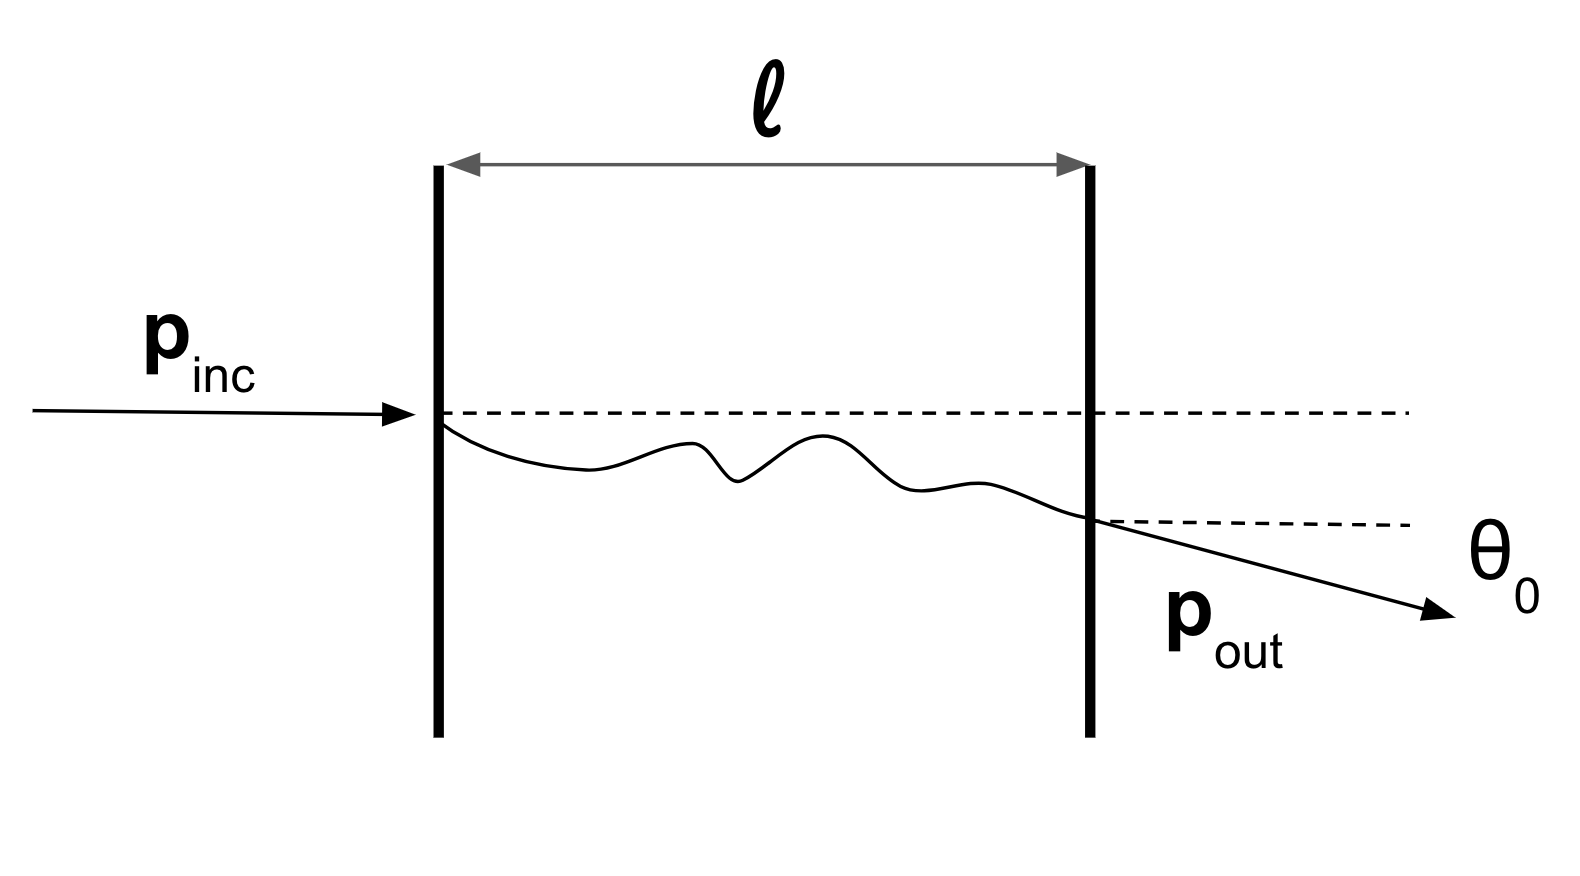
\includegraphics[scale=0.2]{MCS2D}
\caption{2D sketch of MCS.}
\label{fig:MCSModel2D}
\end{figure}

\begin{figure}[hbpt]
\centering
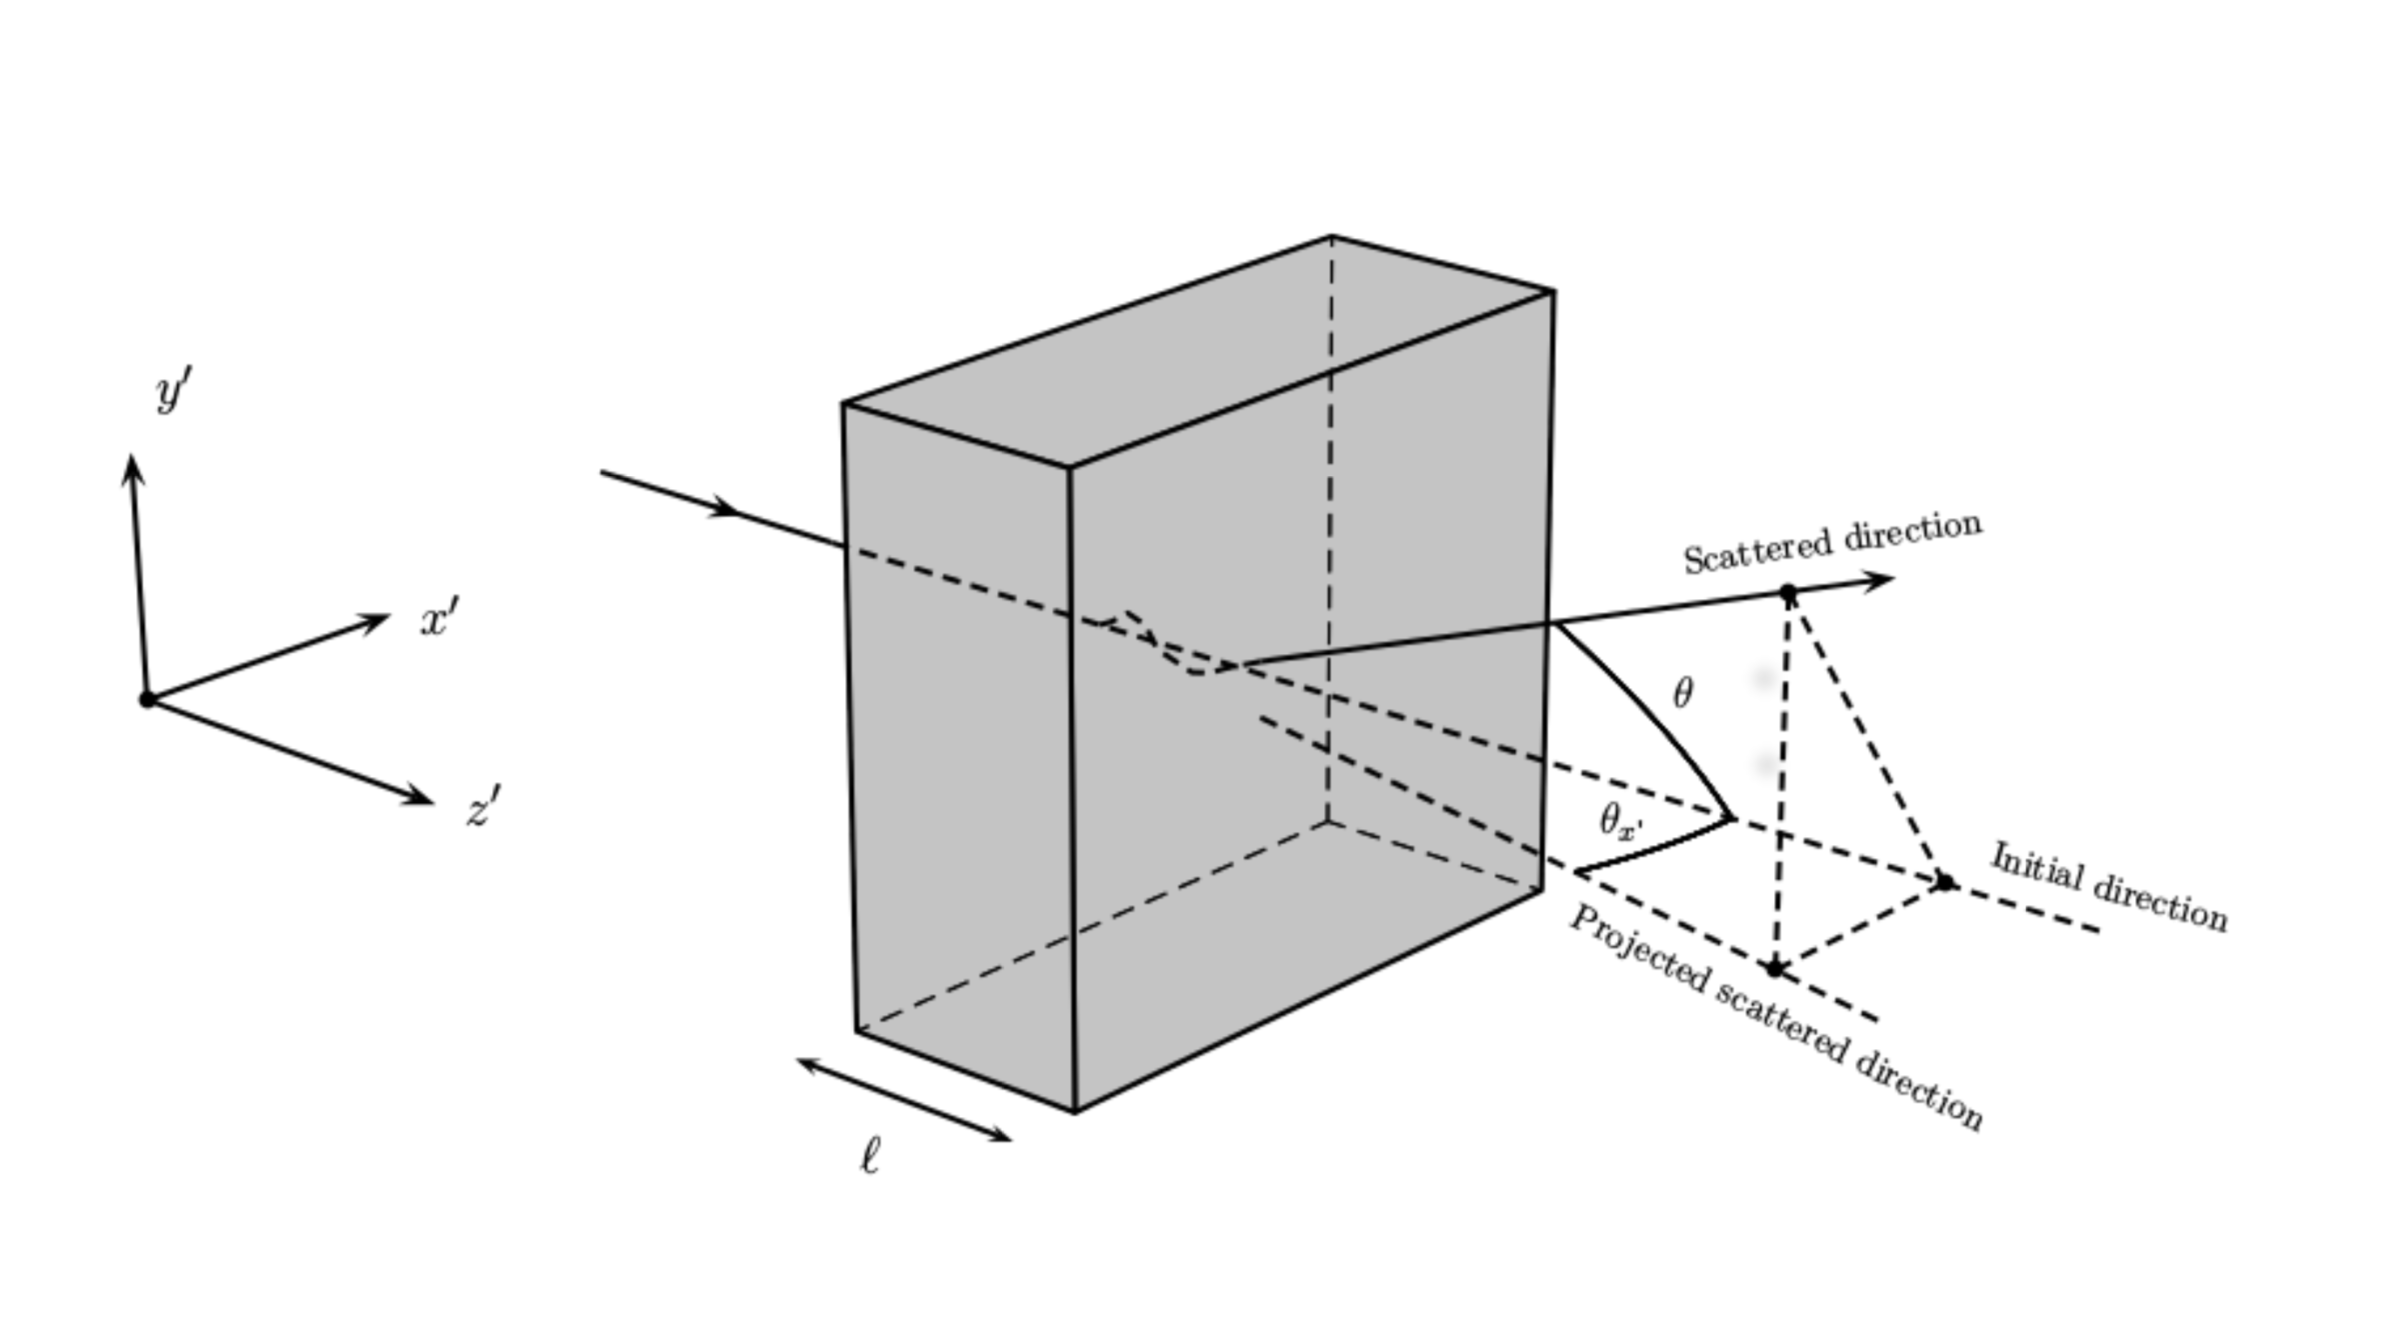
\includegraphics[scale=0.2]{MCS3D}
\caption{3D sketch of MCS.}
\label{fig:MCSModel3D}
\end{figure}

In a more realistic tri-dimensional representation, show in Figure \ref{fig:MCSModel3D} we define  $\theta_x$ and $\theta_y$ as the angle between the projections in the XZ and YZ planes. These angles are both distributed as  gaussians centered at zero and standard deviation $\sigma_{MSC}$, in symbols:
\begin{equation}
\theta_{x} \sim \mathcal N (0, \sigma_{MSC}^2) \text{ and } \theta_{y} \sim \mathcal N (0, \sigma_{MSC}^2).
\end{equation}
For small angles,  we can approximate the 3D angle between the incoming and outgoing momenta as 
\begin{equation}
\theta_{3D} = \sqrt{ \theta_x^2 + \theta_y^2}.
\end{equation}
Thus, we can assume that $\theta_{3D}^2$ is distributed as the sum of two independent gaussian distributions with the same mean $\mu_x=\mu_y=0$ and same standard deviation $\sigma_x=\sigma_y=\sigma_{MCS}$; in symbols,
\begin{equation}
\theta^2_{3D} = \sum_{i=x,y}\theta^2_i \sim \sum_{i=x,y}\Gamma(1/2, 2\sigma_i^2) = \Gamma(n/2, 2\sigma^2_{MCS}),
\end{equation} 
where $n$ is the number of gaussian-distributed variables in the sum (in our case $n=2$) and $\Gamma$ is the gamma distribution. Substituting $n$, we simply find 
\begin{equation}
\theta^2_{3D}  \sim  \Gamma(1, 2\sigma^2_{MCS}). 
\end{equation} 
A common analytical parametrization of the gamma distribution in the $k$ and $\alpha$ parameters is as follows:
\begin{equation}
\Gamma(k, \alpha) = \frac{1}{\Gamma(k) \alpha^k}x^{k-1}e^{-\frac{x}{\alpha}}, 
\end{equation} 
where $\Gamma(k)$ is the nicely confusing gamma function, i.e. the compact version of the factorial, $\Gamma(k) = (k-1)!$  -- don't you love statisticians?   \\
In our case, the form of the gamma distribution is greatly simplified by the fact that $k=1$. In fact, $\Gamma(1) = 1$, $x^{k-1} = x^0 = 1$ and the gamma function  becomes:

\begin{equation}
\theta^2_{3D}  \sim \Gamma(1, 2\sigma^2_{MCS}) = \frac{1}{2\sigma^2_{MCS}}e^{-\frac{\theta^2_{3D} }{2\sigma^2_{MCS}}}. 
\end{equation} 


In order to calculate the Highland formula as a function of the momentum, we divide the LArIAT events in bins of incident momentum and we measure $\sigma_{MCS}$ in each bin. For each bin, we plot the $\theta^2_{3D}$ distribution, we fit it with an exponential and we find the slope; then we calculate $\sigma_{MCS}\pm\delta\sigma_{MCS}$ from the estimated slope and the fit uncertainty.

The form of the function used to fit the $\theta^2_{3D}$ distributions is the following
\begin{equation}
\theta^2_{3D}  \sim   C e^{\alpha \theta^2_{3D}},
\end{equation}
where $C$ is a normalization factor and $\alpha = -\frac{1}{2\sigma^2_{MCS}}$. Thus, accounting for the propagation of uncertainties, we find

\begin{equation}
\sigma_{MCS} \pm \delta \sigma_{MCS}=  \sqrt{ -\frac{1}{2\alpha} } \pm \sigma_{MCS} \frac{\delta\alpha}{2\alpha},
\end{equation}
where $\delta\alpha$ is the uncertainty of the fit parameter.


\section{\label{sec:Method}  Measurement Methodology}
\textcolor{red}{How are we measuring it?}


\section{\label{sec:ResultsMu} Results}
% sections are not used for PRL papers




\input acknowledgement.tex   % input acknowledgement

\begin{thebibliography}{99}

  \bibitem{LArIATDet}
    Standard LArIAT detector reference:  \\
R. Acciarri {\sl et al.} (LArIAT Collaboration),
hopefully we'll have one soon.

 \end{thebibliography}

\end{document}
%
% ****** End of file template.aps ******
